\section{Process}
\subsection{Overview}
\label{Overview}
In order to take full advantage of the tools employed in this project as well as the opportunity to work at the hospital, an iterative and incremental user driven development process was chosen. This allowed the student to take advantage of the tacit knowledge of clinical staff and allowed the end-user to actively participate in the design of the system. The iterative and incremental nature of the process allowed the student to start with one form and then incrementally add more forms as well as managing iterative changes in existing forms through user feedback. The ultimate goal of any project is to supply an outcome that will be accepted by the stakeholders, in this case the end users. User driven development enabled the designer to ensure that during all steps in the project the system met stakeholder needs and requirements. The active feedback gained from clinical staff enabled the designer to shape and form the system to meet user needs. It is important to note that sitting down with clinical staff was not always possible as their priority lies with patient care. In order to facilitate a continued design process throughout the semester a number of methods were employed. The student utilised participative observations, interviews as well as feedback notes to gain an adequate understanding of the user needs and requirements. The student's work at the SAN was supported by a project manager from the SAN, Hannah Chong, that facilitated first meetings with clinical staff as well as offering feedback on relevant project management aspects of the project.

\subsubsection{Participative Observations}
As this was the first time the designer had undertaken a IT project within the health domain it was important to learn how clinical staff worked. Participative observations facilitated this need through \emph{shadowing} clinical staff during various points in their shift. This included sitting in on clinical handover, the process through which the nurse of the previous shift conveys patient information to the nurses of the oncoming shift. By sitting in on handover the designer was able to gain an understanding of the overall process of clinical handover as well as experience the shortcomings and inefficiencies first hand. This enabled the designer to relate to the clinical staff when discussing the system design. 
\\ \\
The designer did not actively participate in handover, that is to say that the designer merely observed and did not give handover. Thus, the designer acted like a `fly on the wall', remaining in the background looking on. This method proved vital to the project as it provided a first hand experience of the current situation. One disadvantage of using participative observations was that the designer was overwhelmed at first by the sheer amount of information that he was exposed to. It took some time and effort on the part of the designer to sift through, filter and understand the information in order to make the most efficient use of it. As the project progressed this information overload continually decreased.

\subsubsection{User Interviews}
In order to supplement participative observations, user interviews were undertaken with various clinical staff fulfilling different roles within the hospital. This enabled the designer to understand the viewpoints of various staff in regards to what they do as well as their view on clinical handover. The interviews lasted between ten and fifteen minutes and were held casually. During the interviews, the designer asked specific questions about handover and the user's involvement. The interviews were held on the ward or in offices depending on the role of the staff being interviewed. The interviews also served the purpose of building a relationship with the clinical staff. The designer's aim was to go back to the interviewed staff throughout the project and attain their feedback on the system design. This social component was very important in order to elicit staff support especially nursing staff as their time was extremely limited. Not undertaking this social component would have made the work of the designer much more difficult.

\subsubsection{Feedback Notes}
During the course of the project, the designer met with clinical staff at various times in order to show them the current status of the design as well as to get answers to open questions. During each of these encounters, notes were taken in order to preserve the exchange allowing the designer to return to the notes at a later time to refresh his memory. In order to maximise the use of time with the clinical staff the designer was accompanied by a colleague who assisted with taking notes during the feedback sessions. This allowed the designer to focus on the staff and not waste time trying to write down information as well as facilitating a smooth flow during the meetings with staff.

\newpage
\subsection{Tools and Skills}
From the beginning of the project, one of the key aspects was the use of the \gls{iCIMS}.  Having been created recently, the project was meant to trial the tool in a real world scenario. The main ideology behind iCIMS is to use a graphical interface to build a system thus avoiding the necessity for programming skills. This means that end-users could actively participate in designing the system by creating the system together with the designer. iCIMS aims to be applicable in any clinical situation and thus utilises Ockham's Razor of Design (\cite{Budd}), which states that :

\begin{quote}
\center\emph{``a design should use the minimal number of entities \\ with their maximal generalisations"}
\end{quote}
\vspace{6mm}
\noindent In conjunction with using iCIMS, the designer utilised Trac, a bug and issue tracking system that also offers documentation functionality in the form of a wiki. Two separate instances of Trac were used because the iCIMS project had an existing instance. All bugs and issues were documented in the iCIMS instance of Trac and all project documentation was created in a separate instance of Trac available for the project. All relevant project information, such as interview notes, process flows, etc., was documented on the Trac instance. Apart from playing a vital role in the completion of the project academically, the wiki will also serve as a starting point for future designers continuing the project. This ensures that the designer's efforts are properly recorded and will allow future designers to more easily find their way on future projects.
\\ \\
Apart from electronic tools, the designer needed to use communication and people skills in order to successfully undertake this project. Communication and people skills played a vital role as the designer was dealing with end-users that were very technology-adverse as well as having a low computer-literacy. Inter-personal skills allowed the designer to find common ground and terminology with which to communicate with end-users. It also allowed the designer to quell most reservations that clinical staff had towards the project or its purpose.

\newpage
\subsection{Scope and Schedule}
Although the project description outlines that the designer undertake a design of the entire multi-disciplinary handover occurring at the SAN, this was deemed too big of a scope to handle within an academic semester. Figure \ref{Clinical Handover Overview - All User Roles} is a depiction that hints at the complexity and size of the entire clinical handover process.

\begin{figure}[hp]
				\centering
				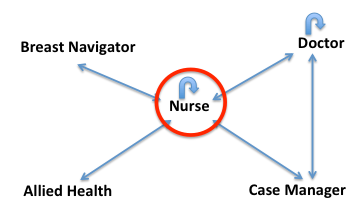
\includegraphics[scale=1.0, width=80mm]{Images/Clinical_Handover_All_Roles}
				\caption{Clinical Handover Overview - All User Roles}
				\label{Clinical Handover Overview - All User Roles}
\end{figure} 

\noindent As shown in figure \ref{Clinical Handover Overview - All User Roles}, there are numerous roles involved in clinical handover each with their own needs and requirements. It was deemed infeasible to undertake requirements analysis, system design and evaluation for all clinical staff involved. The sheer amount of information, communication complexity as well as immense design effort lead to the decision to focus on the nurse role for this project, denoted by the red circle in the figure above. Furthermore, the scope was defined as focusing on the clinical handover between nurses as this was deemed most important in discussions with staff. The nurse to nurse handover is also the most structured handover between clinical staff lending itself to be best suited to this project. 

\newpage 
\noindent With regards to scheduling, the project was divided into four major phases as depicted in figure \ref{Project Process and Schedule}. The week numbers are based on the academic semester timeframe.

\begin{figure}[hp]
				\centering
				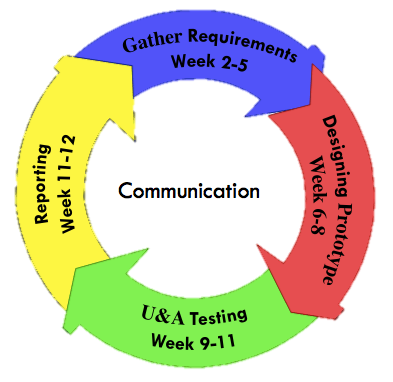
\includegraphics[scale=1.0, width=80mm]{Images/Project_Process}
				\caption{Project Process and Schedule}
				\label{Project Process and Schedule}
\end{figure} 

\noindent Even though the project was divided into four phases, all phases were undertaken in parallel at most times. The separation merely depicts where the focus lay at each point in time. The schedule of four weeks for requirements gathering was a good estimate and allowed the designer to perform an adequate analysis thus enabling the designer to proceed to the design phase. The design phase's projected timeframe of three weeks was too short and was actually the focus of the designer's work until week twelve. This stems from the fact that the designer had numerous issues with the design tool in the form of bugs and it also took longer than expected to convert design ideas into reality within the design tool. This principally because the designer was not familiar with the design tool or its components prior to commencing the project.
\\ \\
Due to the extensive design phase, the usability and acceptance testing phase was pushed back into the weeks twelve and thirteen after the designer was at a point in the design that lent itself to such testing. Although the testing phase timeframe was reduced to two weeks and pushed to the very end of the academic semester, the designer nevertheless managed to obtain testing data in coordination with staff. Due to availability issues with staff, not all clinical staff could undertake the usability and acceptance testing. It should be noted that these availability issues did not stem from bad time or appointment management on behalf of the designer, but rather on issues surrounding staff being sick or having to take personal days off. 
\\ \\
The last phase, the reporting phase, was the focus of week thirteen of the project having been pushed back in order to allow for usability and acceptance testing. This did not pose a major issue as the majority of the reporting phase was in the form of the academic report. The other portion of the reporting phase where the weekly status meetings with Prof. Jon Patrick and the documentation of information in the wiki throughout the semester. At the centre of all phases and indeed of the project lay the communication with clinical staff as well as the project manager Hannah Chong and Prof. Jon Patrick.
